\chapter{Resultados e Discussão}\label{cap:resultados}

Após entender o funcionamento do algoritmo de Viola-Jones e definir a metodologia para análise, foram executadas diversas iterações de classificação sobre o conjunto de imagens, variando os parâmetros de fator de escala para e número mínimo de vizinhos e cada um dos resultados obtidos pode ser exibido como um ponto no espaço ROC obtendo a figura \ref{fig:results_roc}, para que todos sejam facilmente comparados e também se torna simples observar se algum dos resultados está posicionado acima o limite lucrativo traçado. Além das classificações utilizando o classificador de Viola-Jones, foi feita uma classificação utilizando o framework Keras (fonte ref{}) para referência. 

\begin{figure}[htbp]
     \centering
     \caption{Resultados das classificações sobre o espaço ROC. Os parâmetros utilizados em cada resultado são listados na tabela \ref{tab:results_identify}.}
     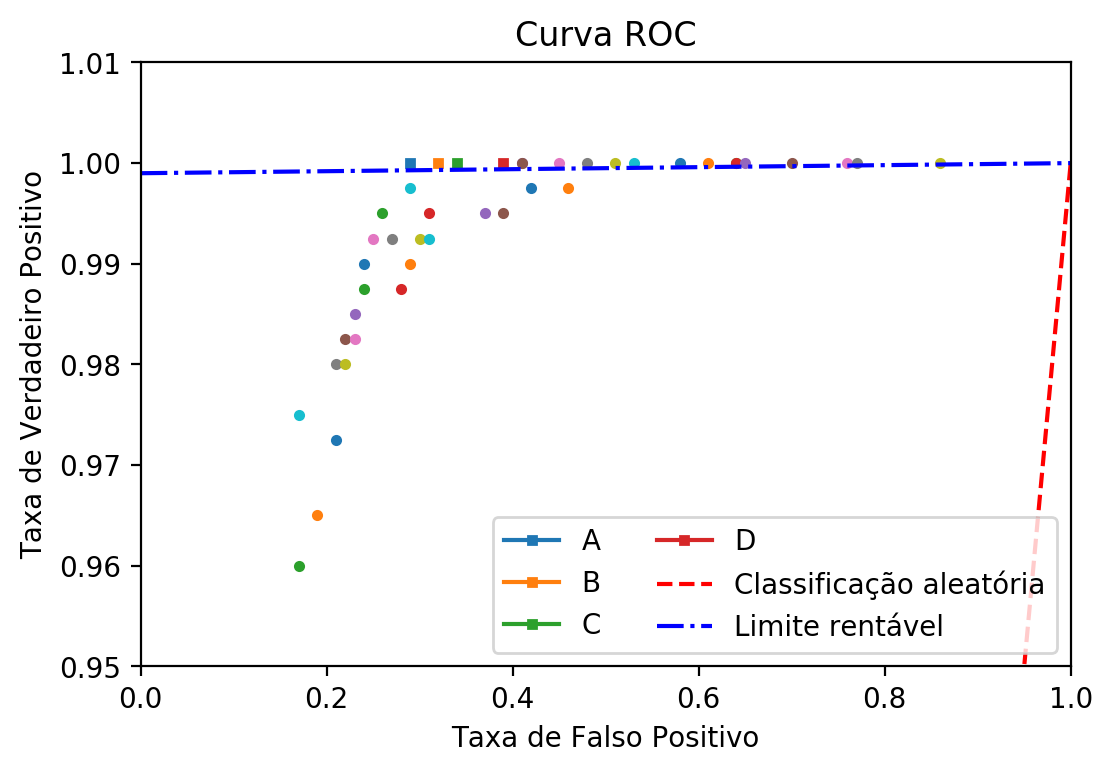
\includegraphics[scale=1]{figs/curva_roc_results.png}
     \label{fig:results_roc}
 \end{figure}

 \begin{table}[htbp]
     \caption{Matriz de confusão com os resultados do primeiro teste.}
     \label{tab:results_identify}
     \centering
     \begin{tabular}{clrr}
      Letra & Método & Fator de Escala & Número Mínimo de Vizinhos \\
      \midrule
           A & OpenCV & 1.30 & 5 \\
           B & OpenCV & 1.30 & 2 \\
           C & OpenCV & 1.05 & 0 \\
           D & OpenCV & 1.05 & 1 \\
           E & OpenCV & 1.05 & 2 \\
           F & OpenCV & 1.05 & 3 \\
           G & OpenCV & 1.05 & 5 \\
           H & Keras & & \\
      \end{tabular}
 \end{table}

Em nenhuma das tentativas de classificação foi obtido um resultado lucrativo. Aprofundando a análise, pode-se observar os resultados de sensitividade, especificidade e acurácia de cada um dos classificadores na tabela \ref{tab:results_data} e a matriz de confusão do resultado que mais se aproximou do cenário lucrativo na tabela ref{}, também foi observado que apenas duas imagens de faces não foram reconhecidas, entre as 17100 testadas.

\begin{table}[htbp]
     \caption{Matriz de confusão com os resultados do primeiro teste.}
     \label{tab:results_data}
     \centering
     \begin{tabular}{crrr}
      Letra & Sensitividade & Especificidade & Acurácia \\
      \midrule
           A & 0.866257 & 0.985497 & 0.890105 \\
           B & 0.933450 & 0.909006 & 0.928561 \\
           C & 0.998480 & 0.129123 & 0.824608 \\
           D & 0.994795 & 0.390877 & 0.874012 \\
           E & 0.990175 & 0.561871 & 0.904515 \\
           F & 0.983509 & 0.668304 & 0.920468 \\
           G & 0.972690 & 0.792281 & 0.936608 \\
           H & 0.936023 & 0.988538 & 0.946526 \\
      \end{tabular}
 \end{table}

Comparando tal resultado com a análise da equação que define o limiar lucrativo da classificação, é possível perceber que cada imagem positiva que é classificada como negativa gera um prejuízo muito elevado, que precisa ser compensado com a classificação correta de uma grande quantidade de imagens negativas. Para o classificador estudado, se torna extremamente difícil atingir tal resultado, mesmo com grande aumento da sensibilidade, classificando quase todas imagens como positivas.

Como uma tentativa extra e com objetivo de comparação, foi utilizado um detector de pele, que se baseia nas cores da imagem, de forma que fosse calculada a quantidade de pele existente em cada imagem, os resultados foram ordenados e então foi traçada a curva ROC na figura \ref{fig:skin_roc} que representa os possíveis limiares da quantidade de pele existente em uma imagem que faria a mesma ser considera como face.

\begin{figure}[htbp]
     \centering
     \caption{Curva ROC para o detector de pele.}
     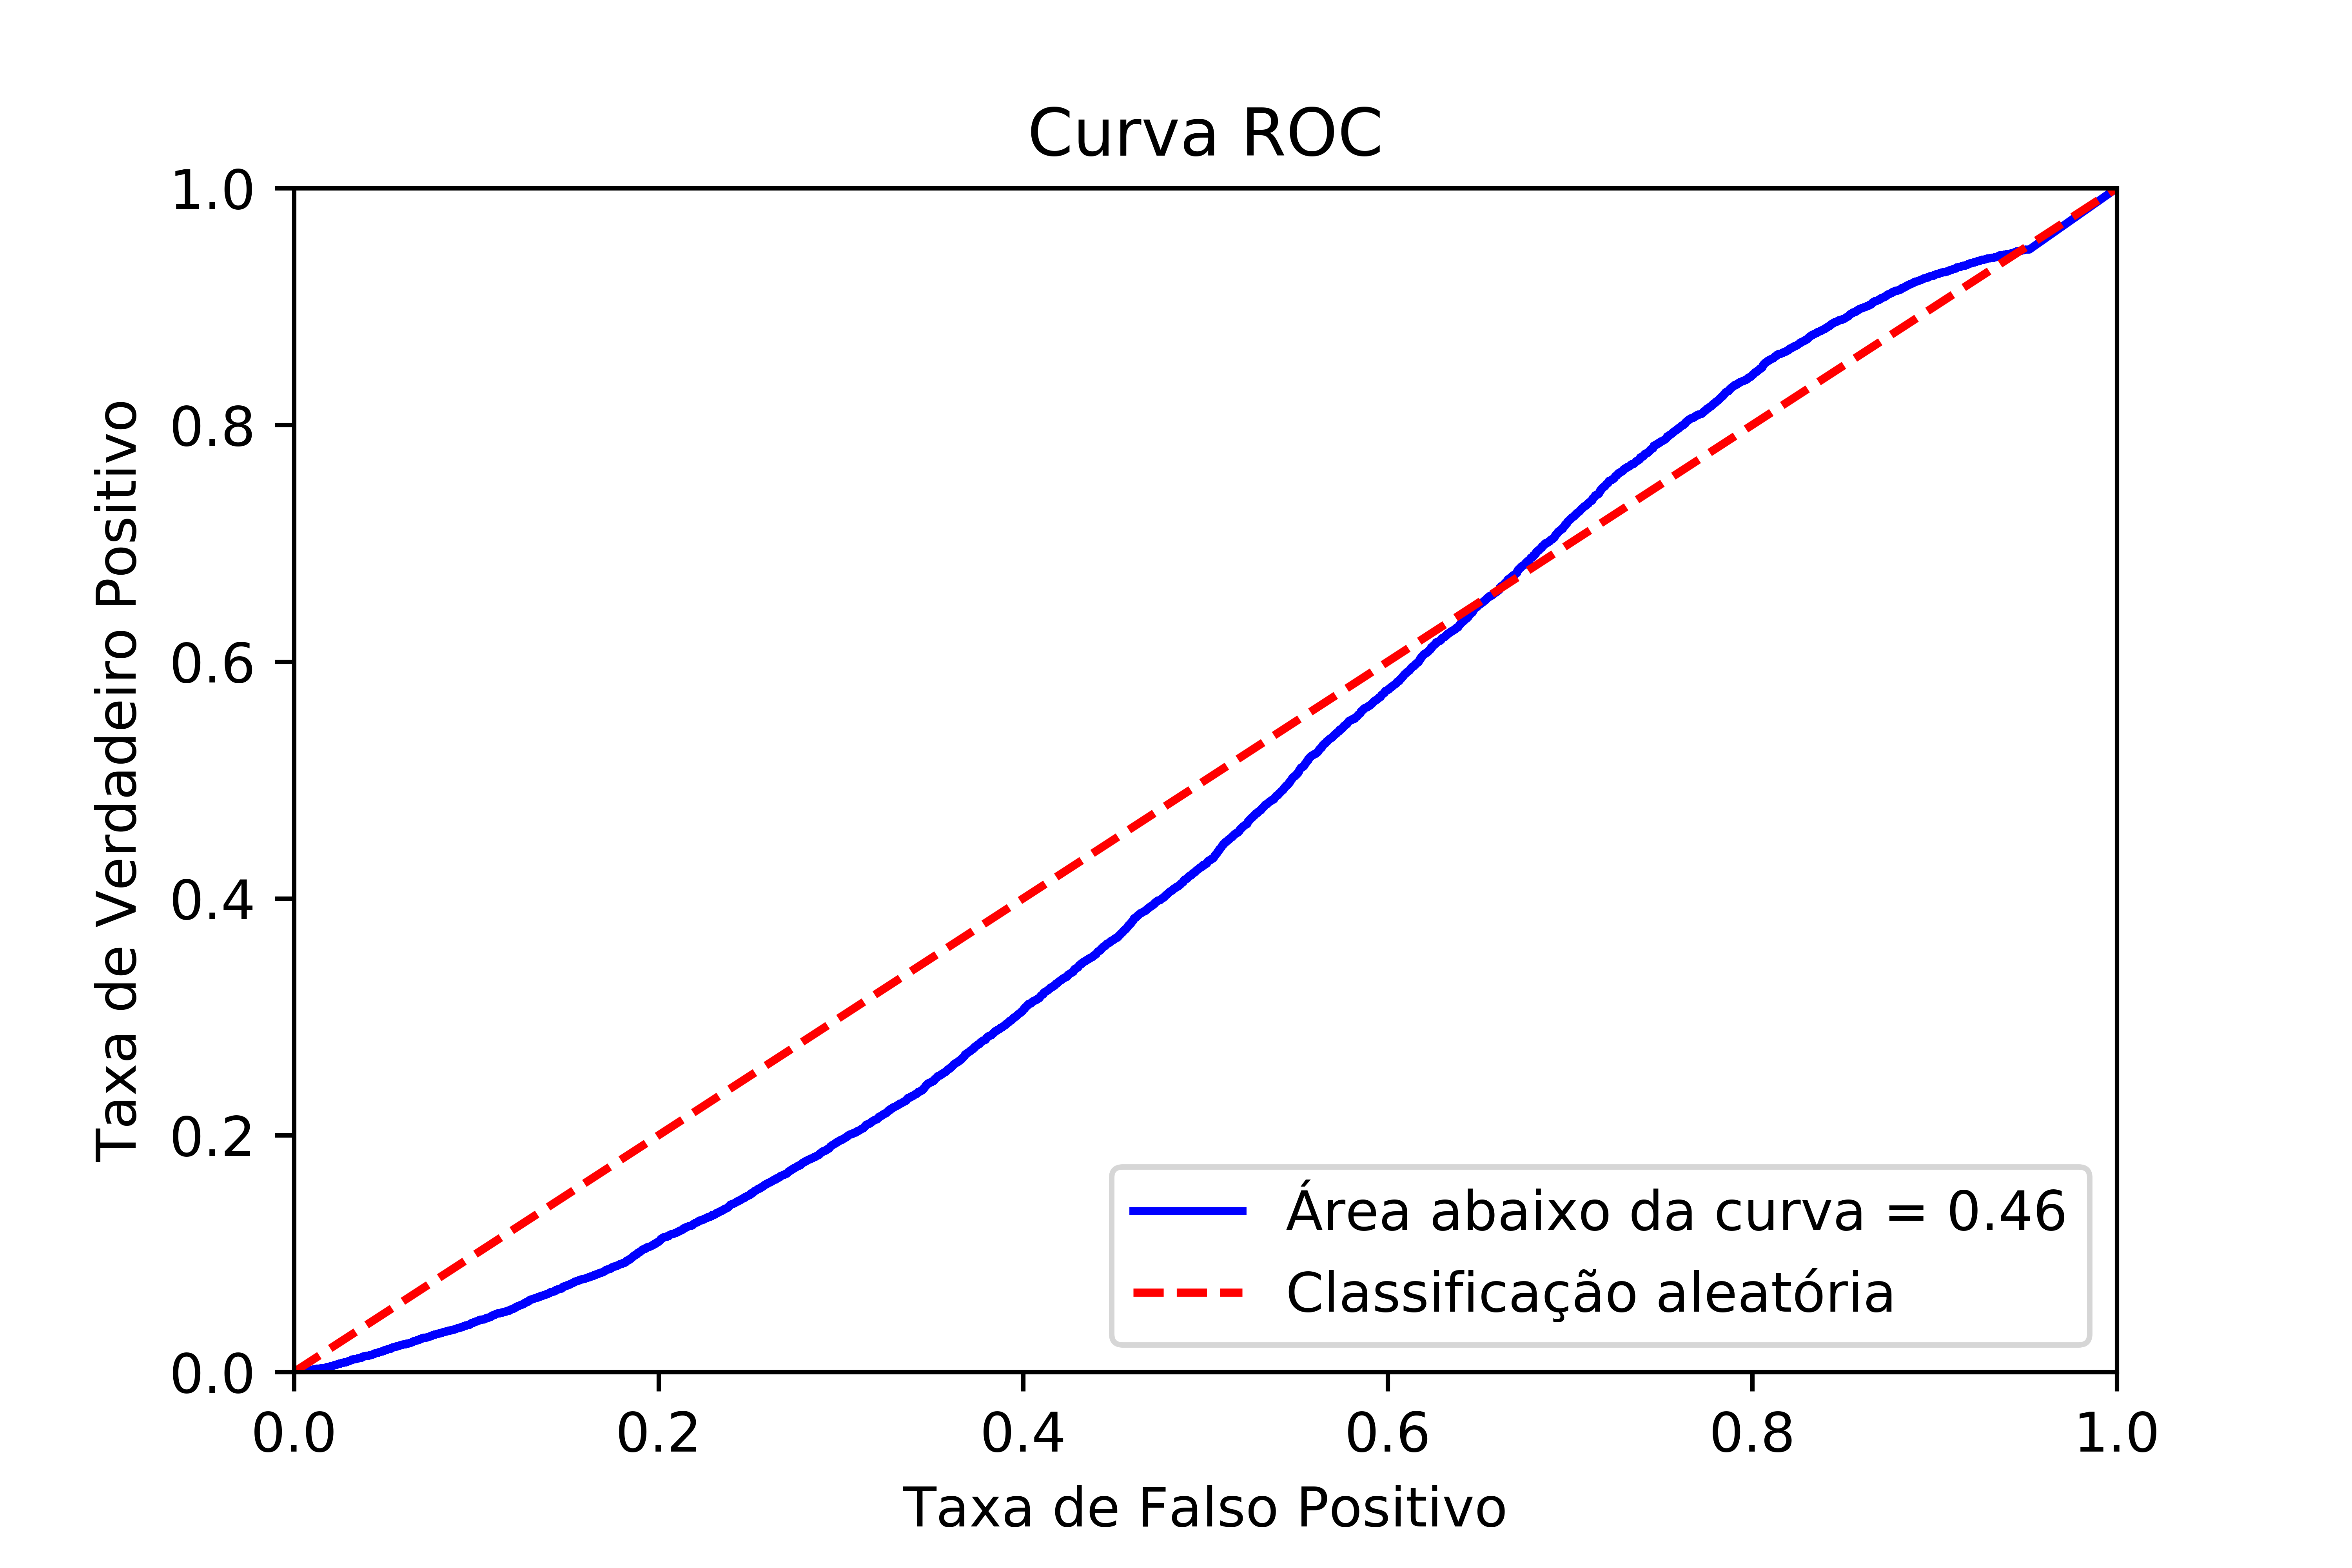
\includegraphics[scale=1]{figs/curva_roc_skin.png}
     \label{fig:skin_roc}
 \end{figure}

A hipótese de que um detector de pele traria bons resultados está relacionada a necessidade de obter um número muito baixo de falsos negativos e a altíssima sensibilidade que é possível obter com tal detector, apesar disso, a quantidade elevada de falsos positivos prejudica bastante os resultados, obtendo um classificador quase igual ao aleatório.
